\chapter{Jet Results and Outlook} \label{ch:cando}

\section{8 TeV Inclusive Jet Results and Discussion}

\subsubsection{Differential Jet Cross-Section}

\afterpage{%

\begin{figure}
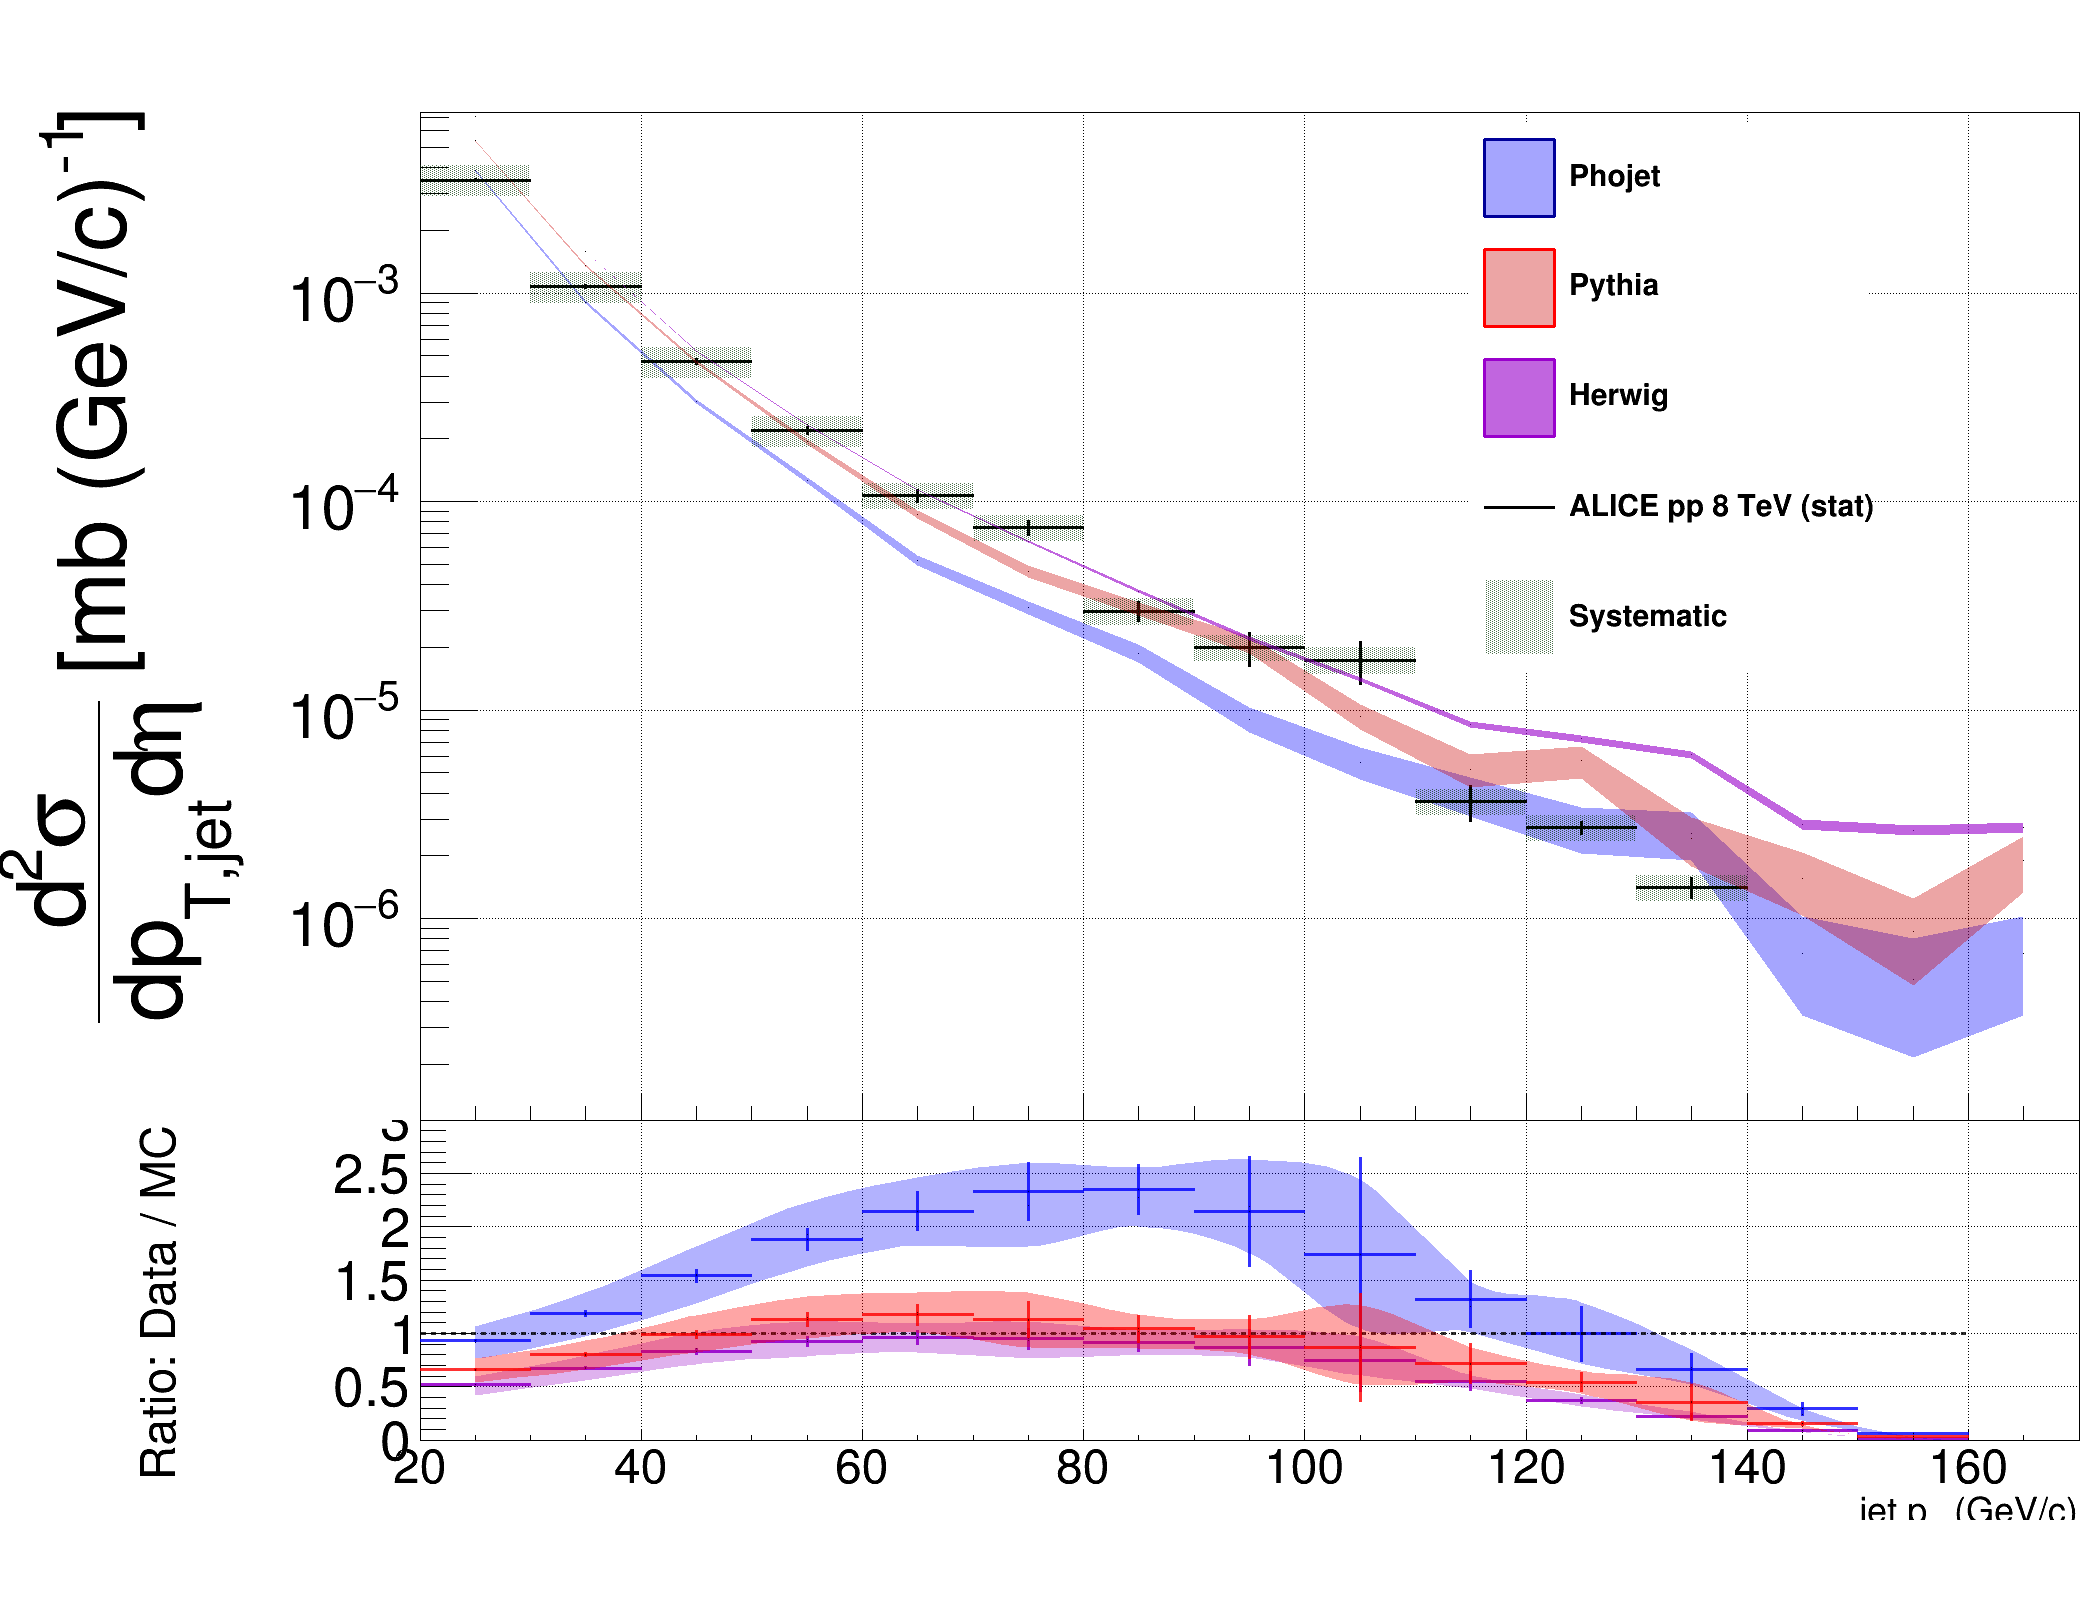
\includegraphics[width=\linewidth]{XSecR02}
\centering
\caption{8 TeV inclusive jet differential cross-section for R = 0.2.}
\label{fig:JetXsecR02}
\end{figure}

\begin{figure}
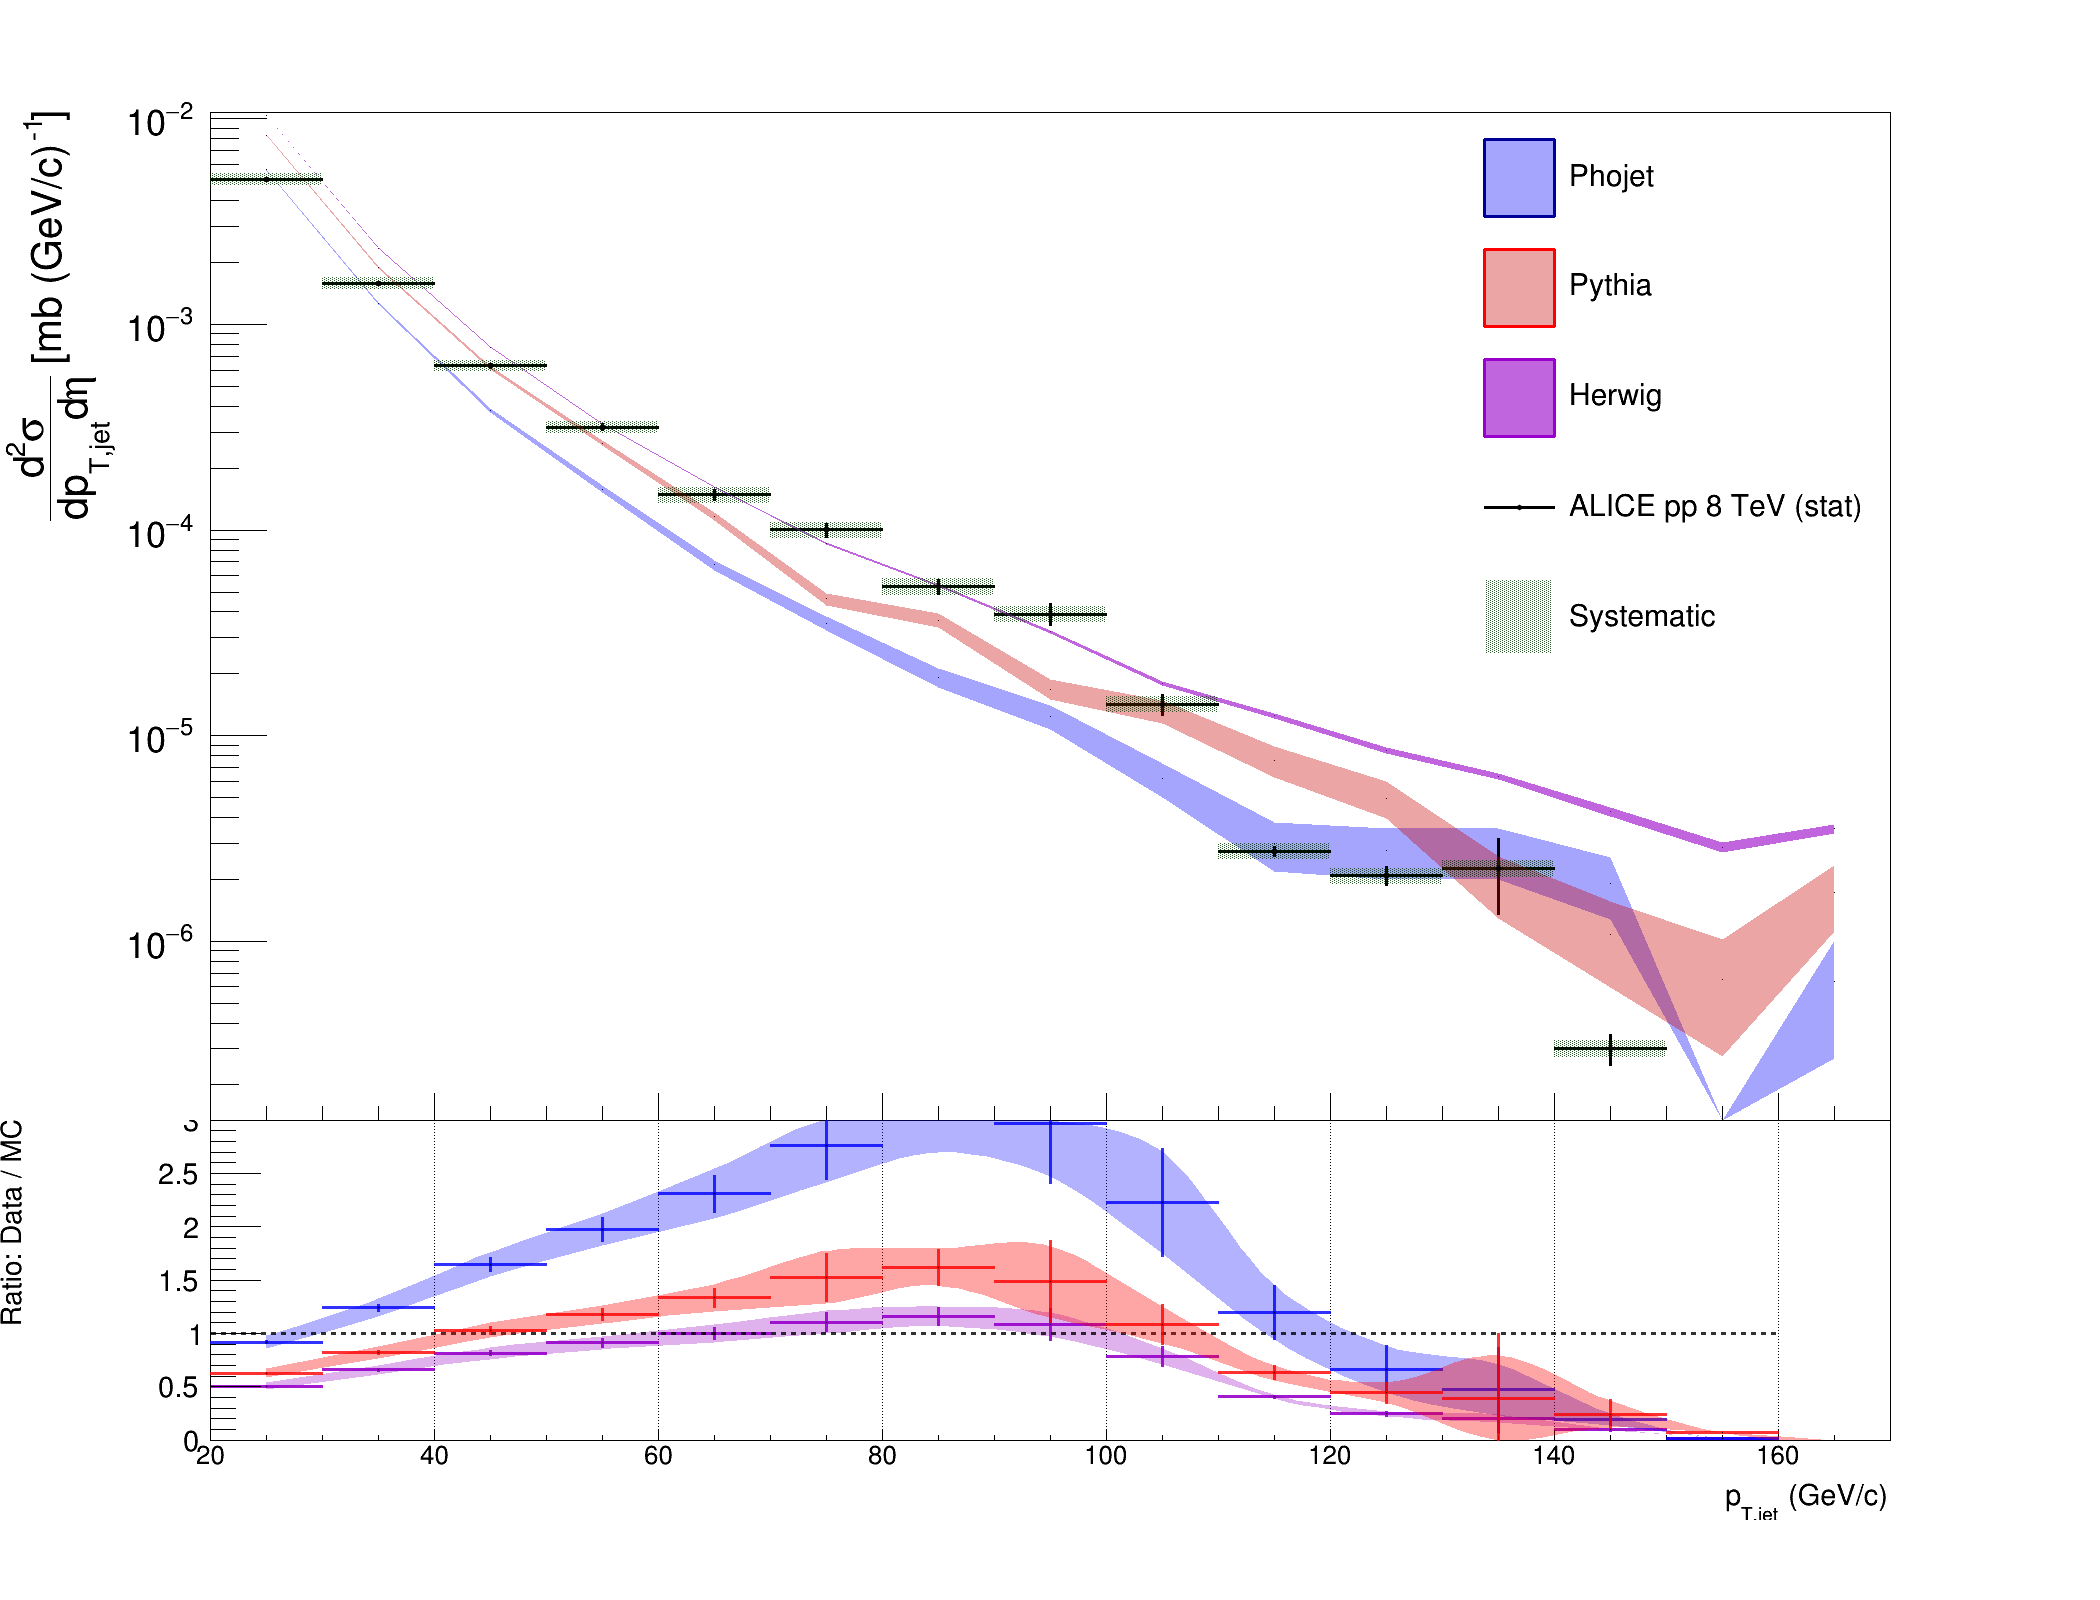
\includegraphics[width=\linewidth]{XSecR03}
\centering
\caption{8 TeV inclusive jet differential cross-section for R = 0.3.}
\label{fig:JetXsecR03}
\end{figure}

\begin{figure}
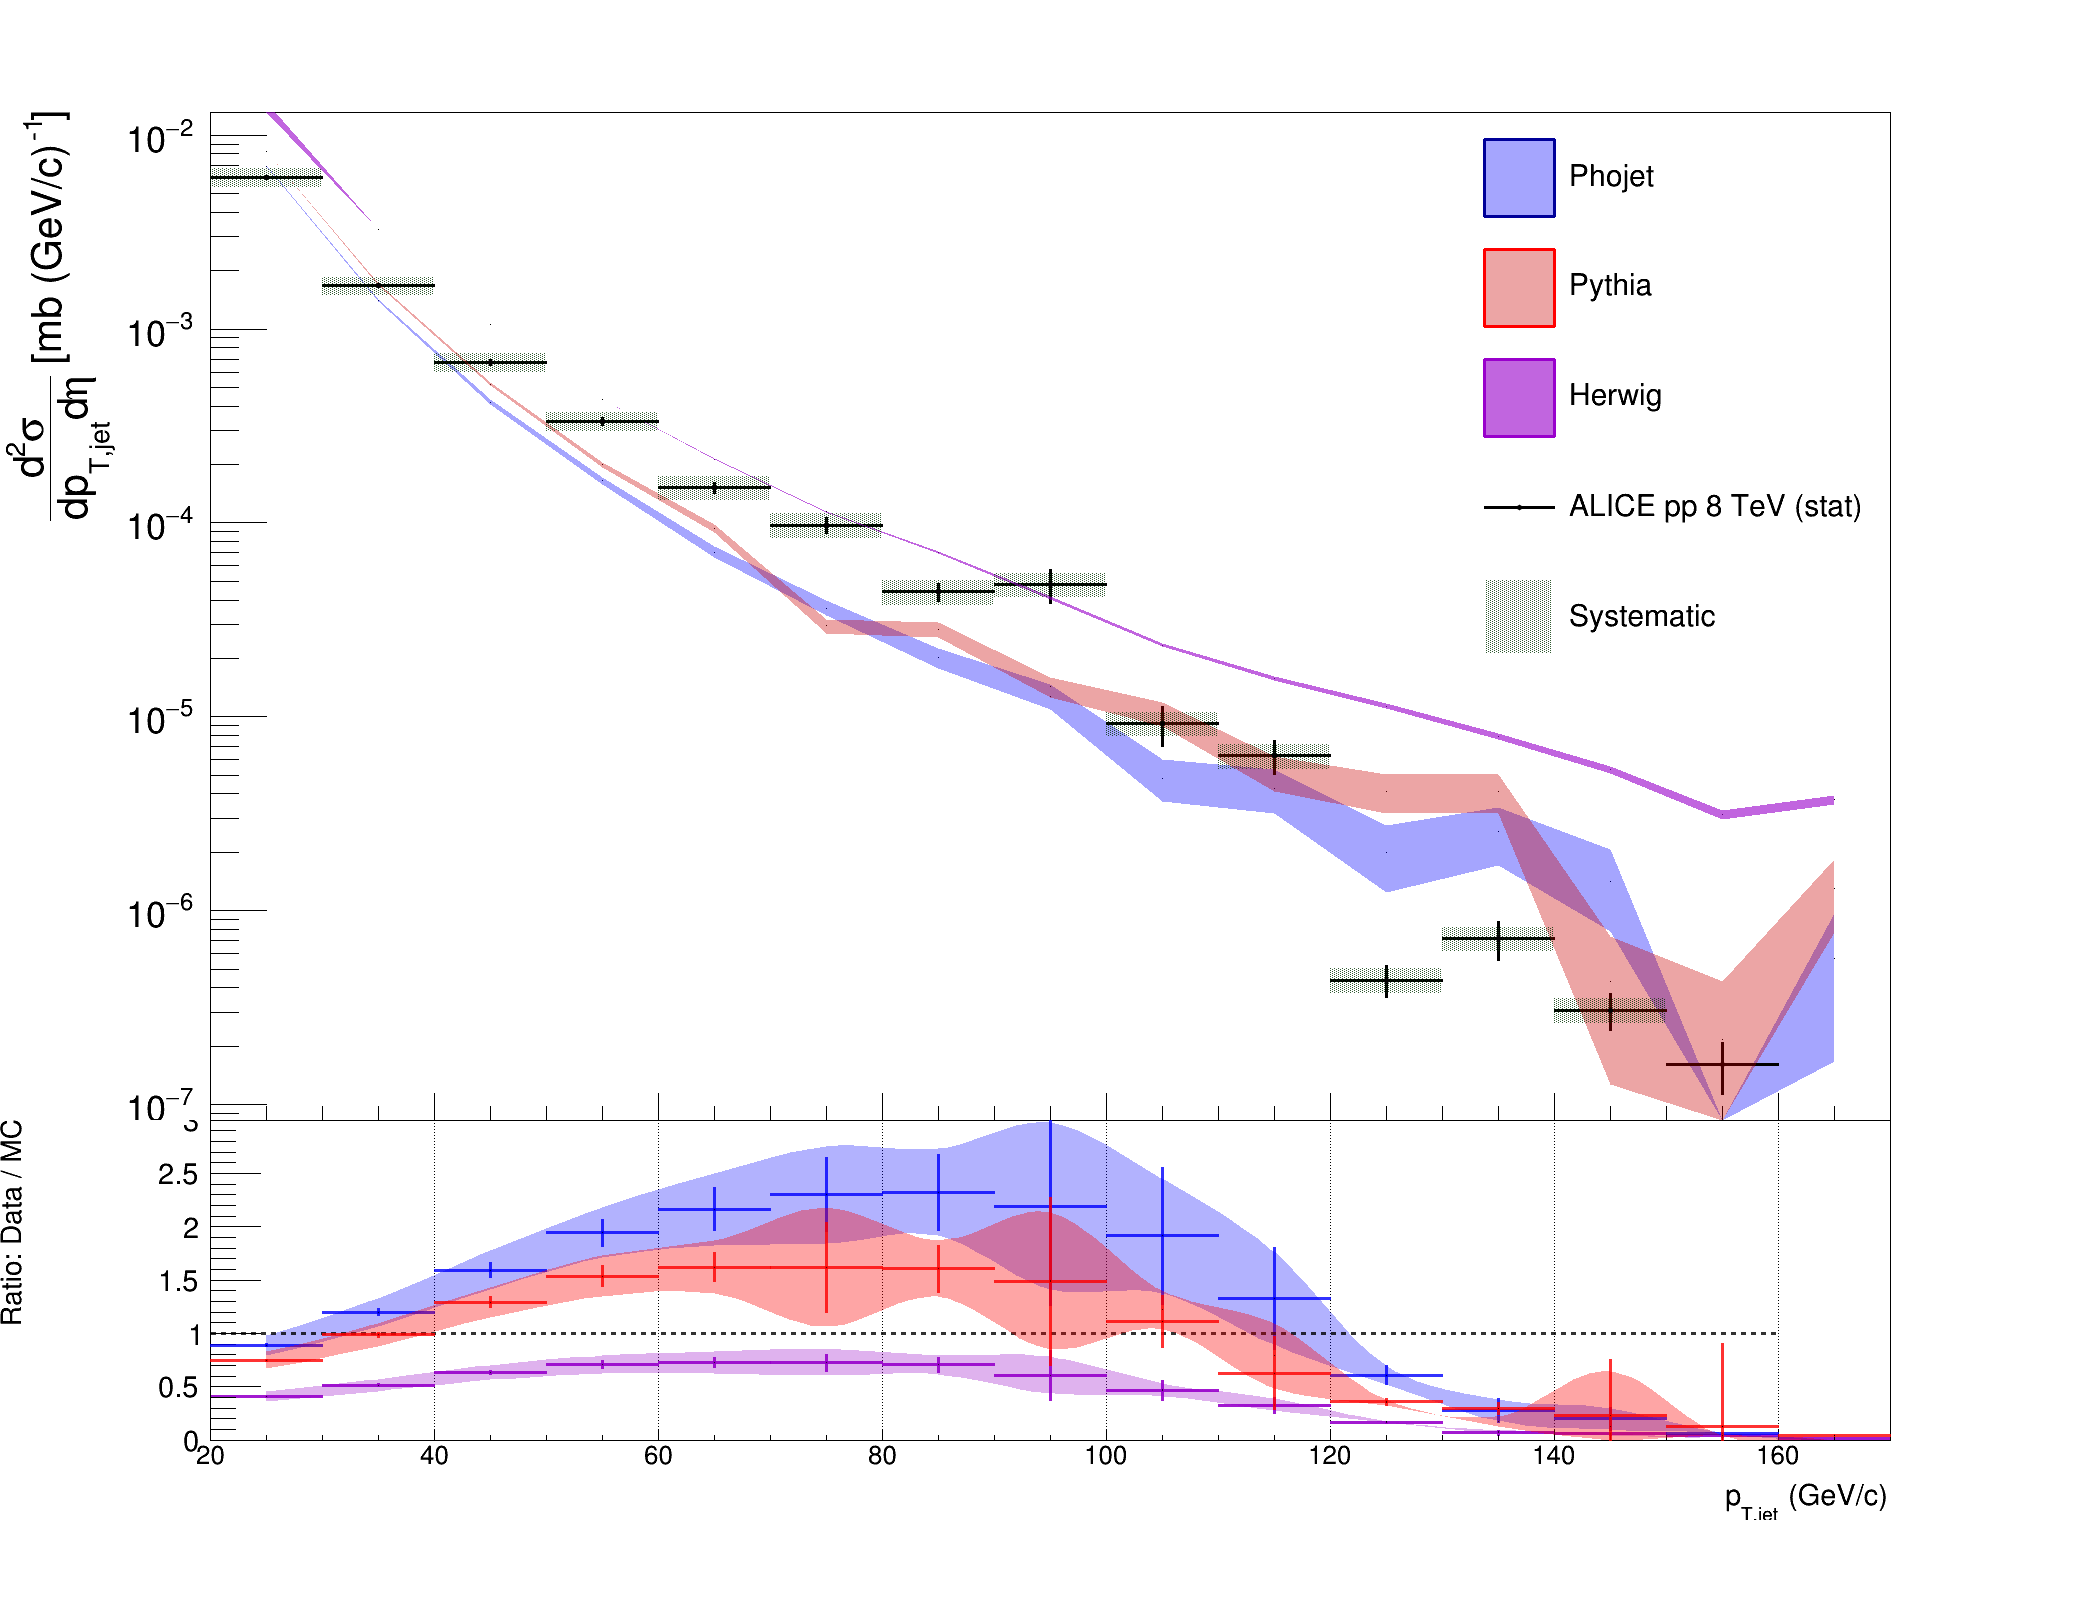
\includegraphics[width=\linewidth]{XSecR04}
\centering
\caption{8 TeV inclusive jet differential cross-section for R = 0.4.}
\label{fig:JetXsecR04}
\end{figure}

\clearpage
}

\noindent
Figures \ref{fig:JetXsecR02}, \ref{fig:JetXsecR03}, and \ref{fig:JetXsecR04} show the inclusive jet cross-sections for radii R = 0.2, R = 0.3, and R = 0.4.  The statistical uncertainty from the relative uncertainty from the response matrix used for the bin-by-bin corrections have been added in quadrature to the statistical uncertainty in the data points.  Only EMCal triggered data is used above 40 GeV/c.  Monte Carlo simulations from PYTHIA, PHOJET, and HERWIG are included and shown as colored solid bands to convey the statistical uncertainties from each simulation.  On the bottom half of each plot are the relative ratios of the ALICE jet cross-sections to one of the Monte Carlos using the same color scheme as above.  

The cross-sections are measured over five orders of magnitude, between 20 GeV/\textit{c} to 160 GeV/\textit{c} in $p_{T}$. The R = 0.2 and R = 0.3 cross-sections show a well defined trend between 20 GeV/\textit{c} - $\sim$120 GeV/c, after which the spectra are dominated by statistical fluctuations.  The fluctuations at high-$p_{T}$ are due to the simulations used  for the bin-by-bin corrections.  

Comparing the results to other CERN experiments is difficult.  ATLAS reported inclusive jet cross-sections from the 8 TeV data for R = 0.4 jets\cite{Aaboud:2017dvo}.  However, ATLAS only performs jet finding down to 100 GeV/\textit{c} and any comparisons are difficult due to the large statistical fluctuations in the highest $p_{T}$ bins from ALICE.  A similar issue exists with jet cross-sections reported by CMS at 8 TeV\cite{CMS:2013kda}.  CMS reports jet cross-sections down to 80 GeV/\textit{c} but only for jets with a radius of R = 0.7.  

Comparing PYTHIA and PHOJET, each tend to underestimate the data.  PHOJET has the least agreement with the data.  The poor agreement with PHOJET can be explained by the fact that PHOJET is an older Monte Carlo generator and better tuned to lower energy experiments.  PHOJET may also be under estimating the data because it focuses on describing photon interactions.  

150 million HERWIG events were generated to compare with the 8 TeV data.  As discussed in Chapter \ref{ch:qcd}, HERWIG is similar to PYTHIA but differs in using the clusterization model for hadronization.  The HERWIG simulation tends to slightly over estimate the data. 

Both HERWIG and PYTHIA agree well with the data between 20 GeV/c to 100 GeV/c.  It is hard to say that one is `better' than the other because of the relatively large statistical errors from PYTHIA.  However, for the R = 0.4 jet cross-section we can see that the data seems to agree better with the clusterization description of hadronization used in HERWIG.  HERWIG better predicts QCD radiation\cite{Bahr:2009ek} and this could account for the agreement with the data.  At large jet radii hadronization should be a smaller effect.  The better agreement seen for R = 0.4 with HERWIG is because it models QCD better than PYTHIA or PHOJET.

These results help to further our understanding of jets and the QCD pheonmena behind them.  Through scaling, these results may serve as a reference for heavy-ion collisions and help to improve our understanding of parton energy loss mechanisms in the QGP.  


\subsubsection{Jet Cross-Section Ratios}


\noindent
The ratio of the jet cross-sections as a function of the jet radii is defined as,

\begin{equation}
\mathscr{R} (p_{T}; \, R_{1},R_{2}) = \frac{d\sigma(R_{1}) /d\eta \, dp_{T} }{d\sigma (R_{2}) /d\eta \, dp_{T}},
\label{eq:jetxsecratio}
\end{equation}

\noindent
where $R_{1}$ and $R_{2}$ are the jet radii. This probes the transverse structure of jets and is sensitive to QCD hardonization\cite{SOYEZ201159}.  Figures \ref{fig:JetXsecRatioR02}, \ref{fig:JetXsecRatioR03}, and \ref{fig:JetXsecRatioR023} report the ratios of the jet cross-sections between R = 0.2 / R = 0.4, R = 0.3 / R= 0.4, and R = 0.2 / R = 0.3 respectively.  The figures show the relative ratios plotted from the 8 TeV ALICE data, PYTHIA, PHOJET, and HERWIG.  Errors between the cross-sections of different radii were considered uncorrelated.  In order to avoid double counting by sampling the same jet found using different radii parameters I used disjointed samples of the 8 TeV data to generate each of the ratio plots.

\afterpage{%

\begin{figure}
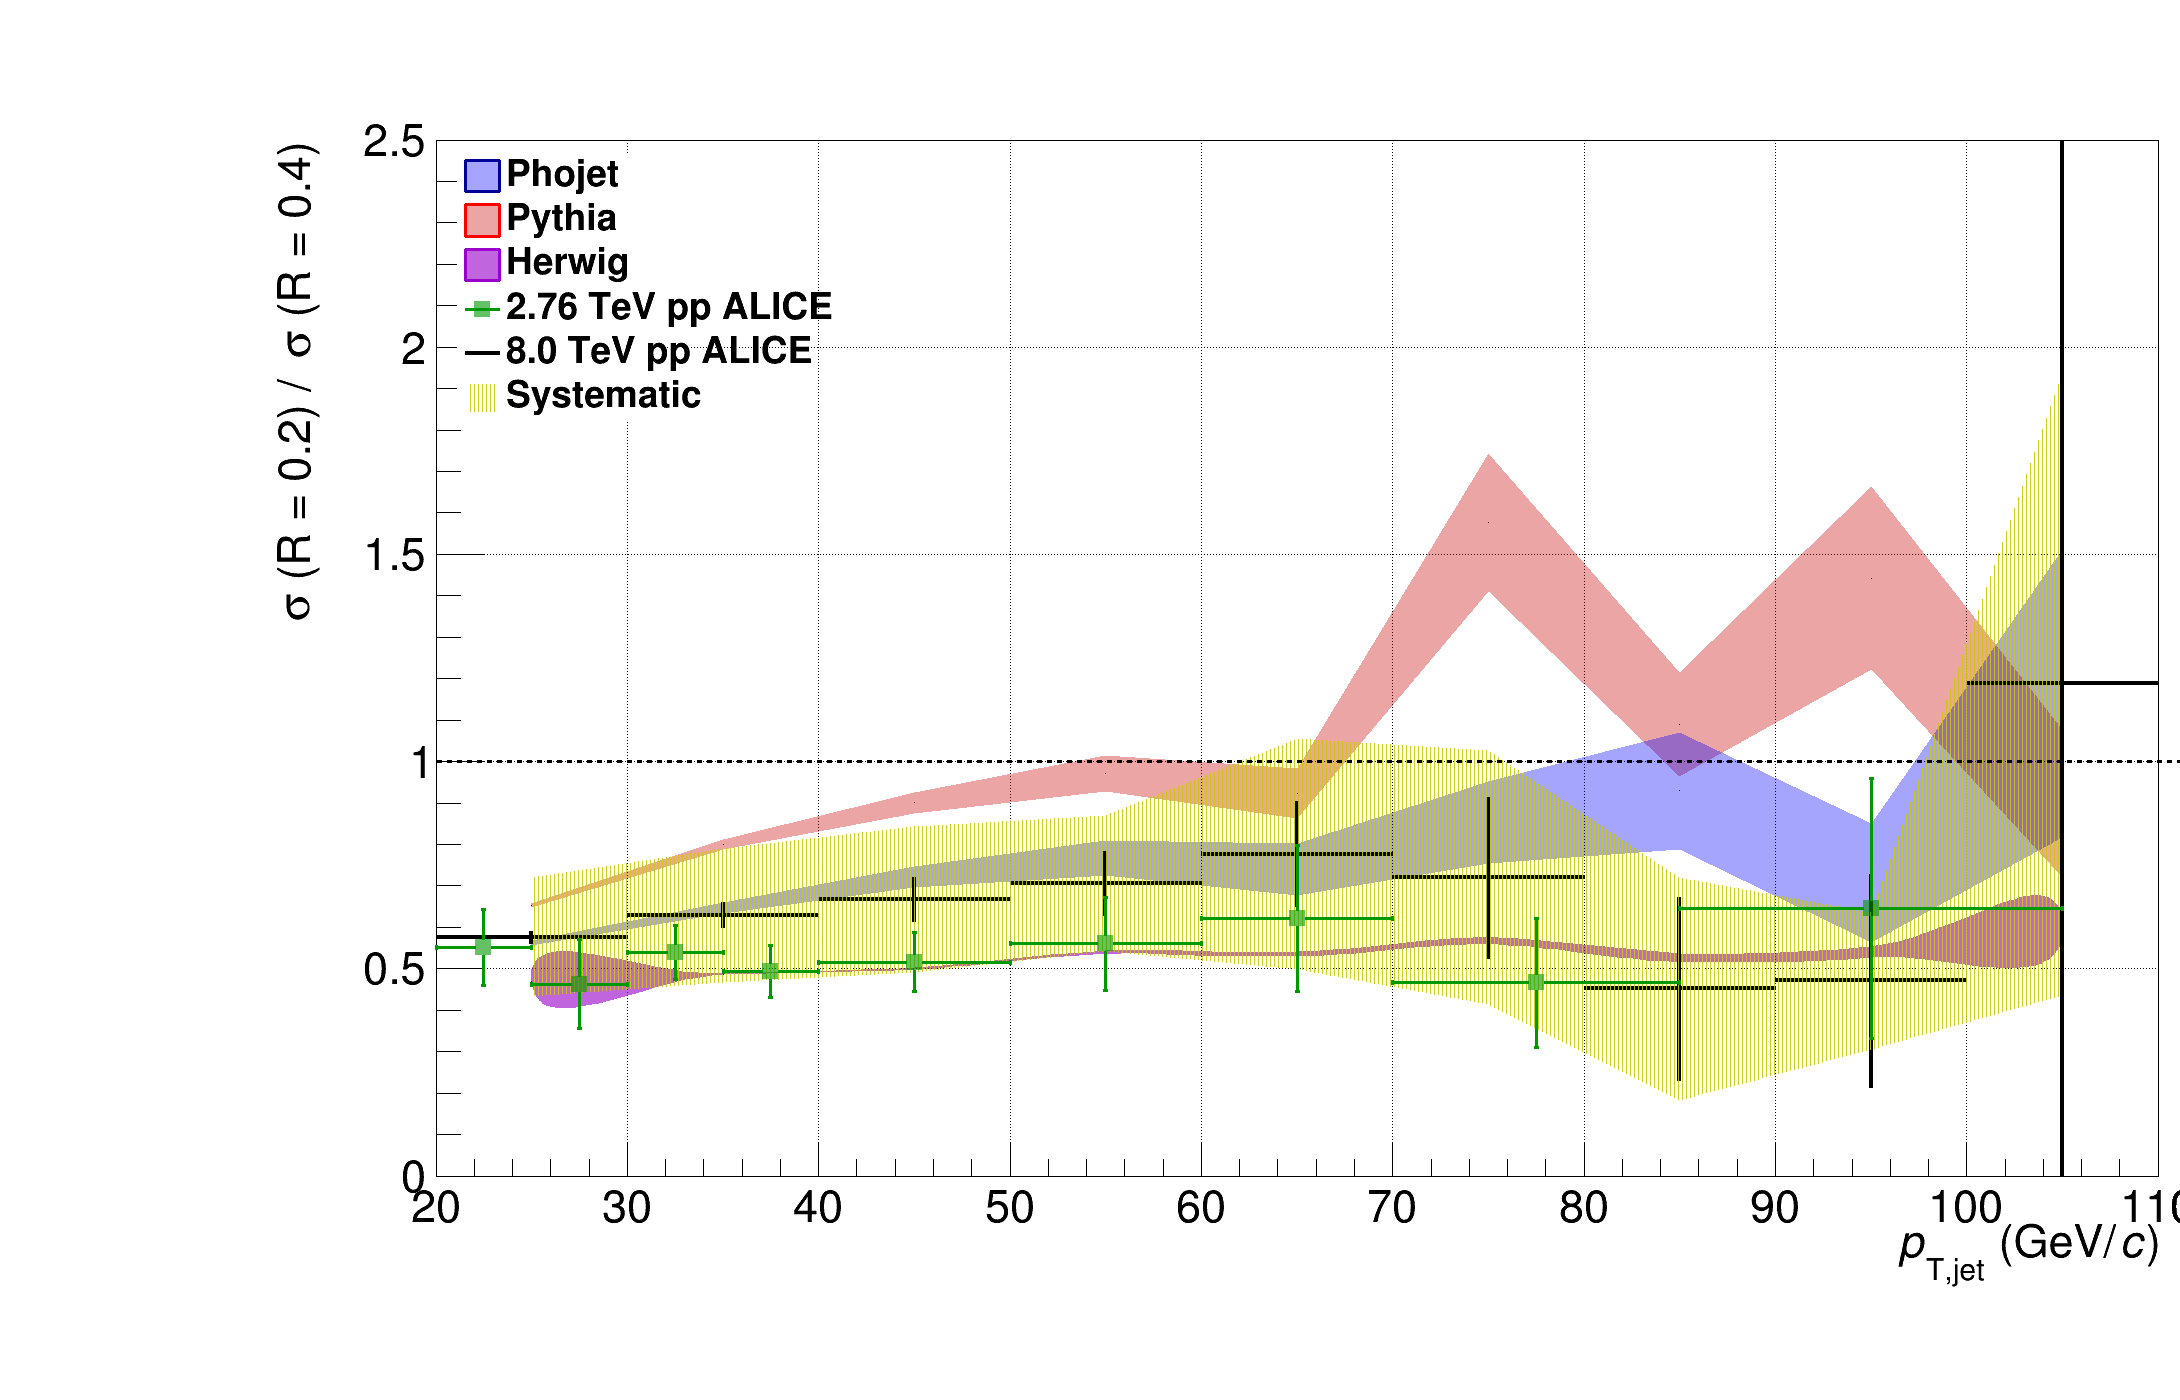
\includegraphics[width=\linewidth]{XSecRatioR02}
\centering
\caption{Ratio of the jet cross-sections R = 0.2  to R = 0.4.}
\label{fig:JetXsecRatioR02}
\end{figure}

\begin{figure}
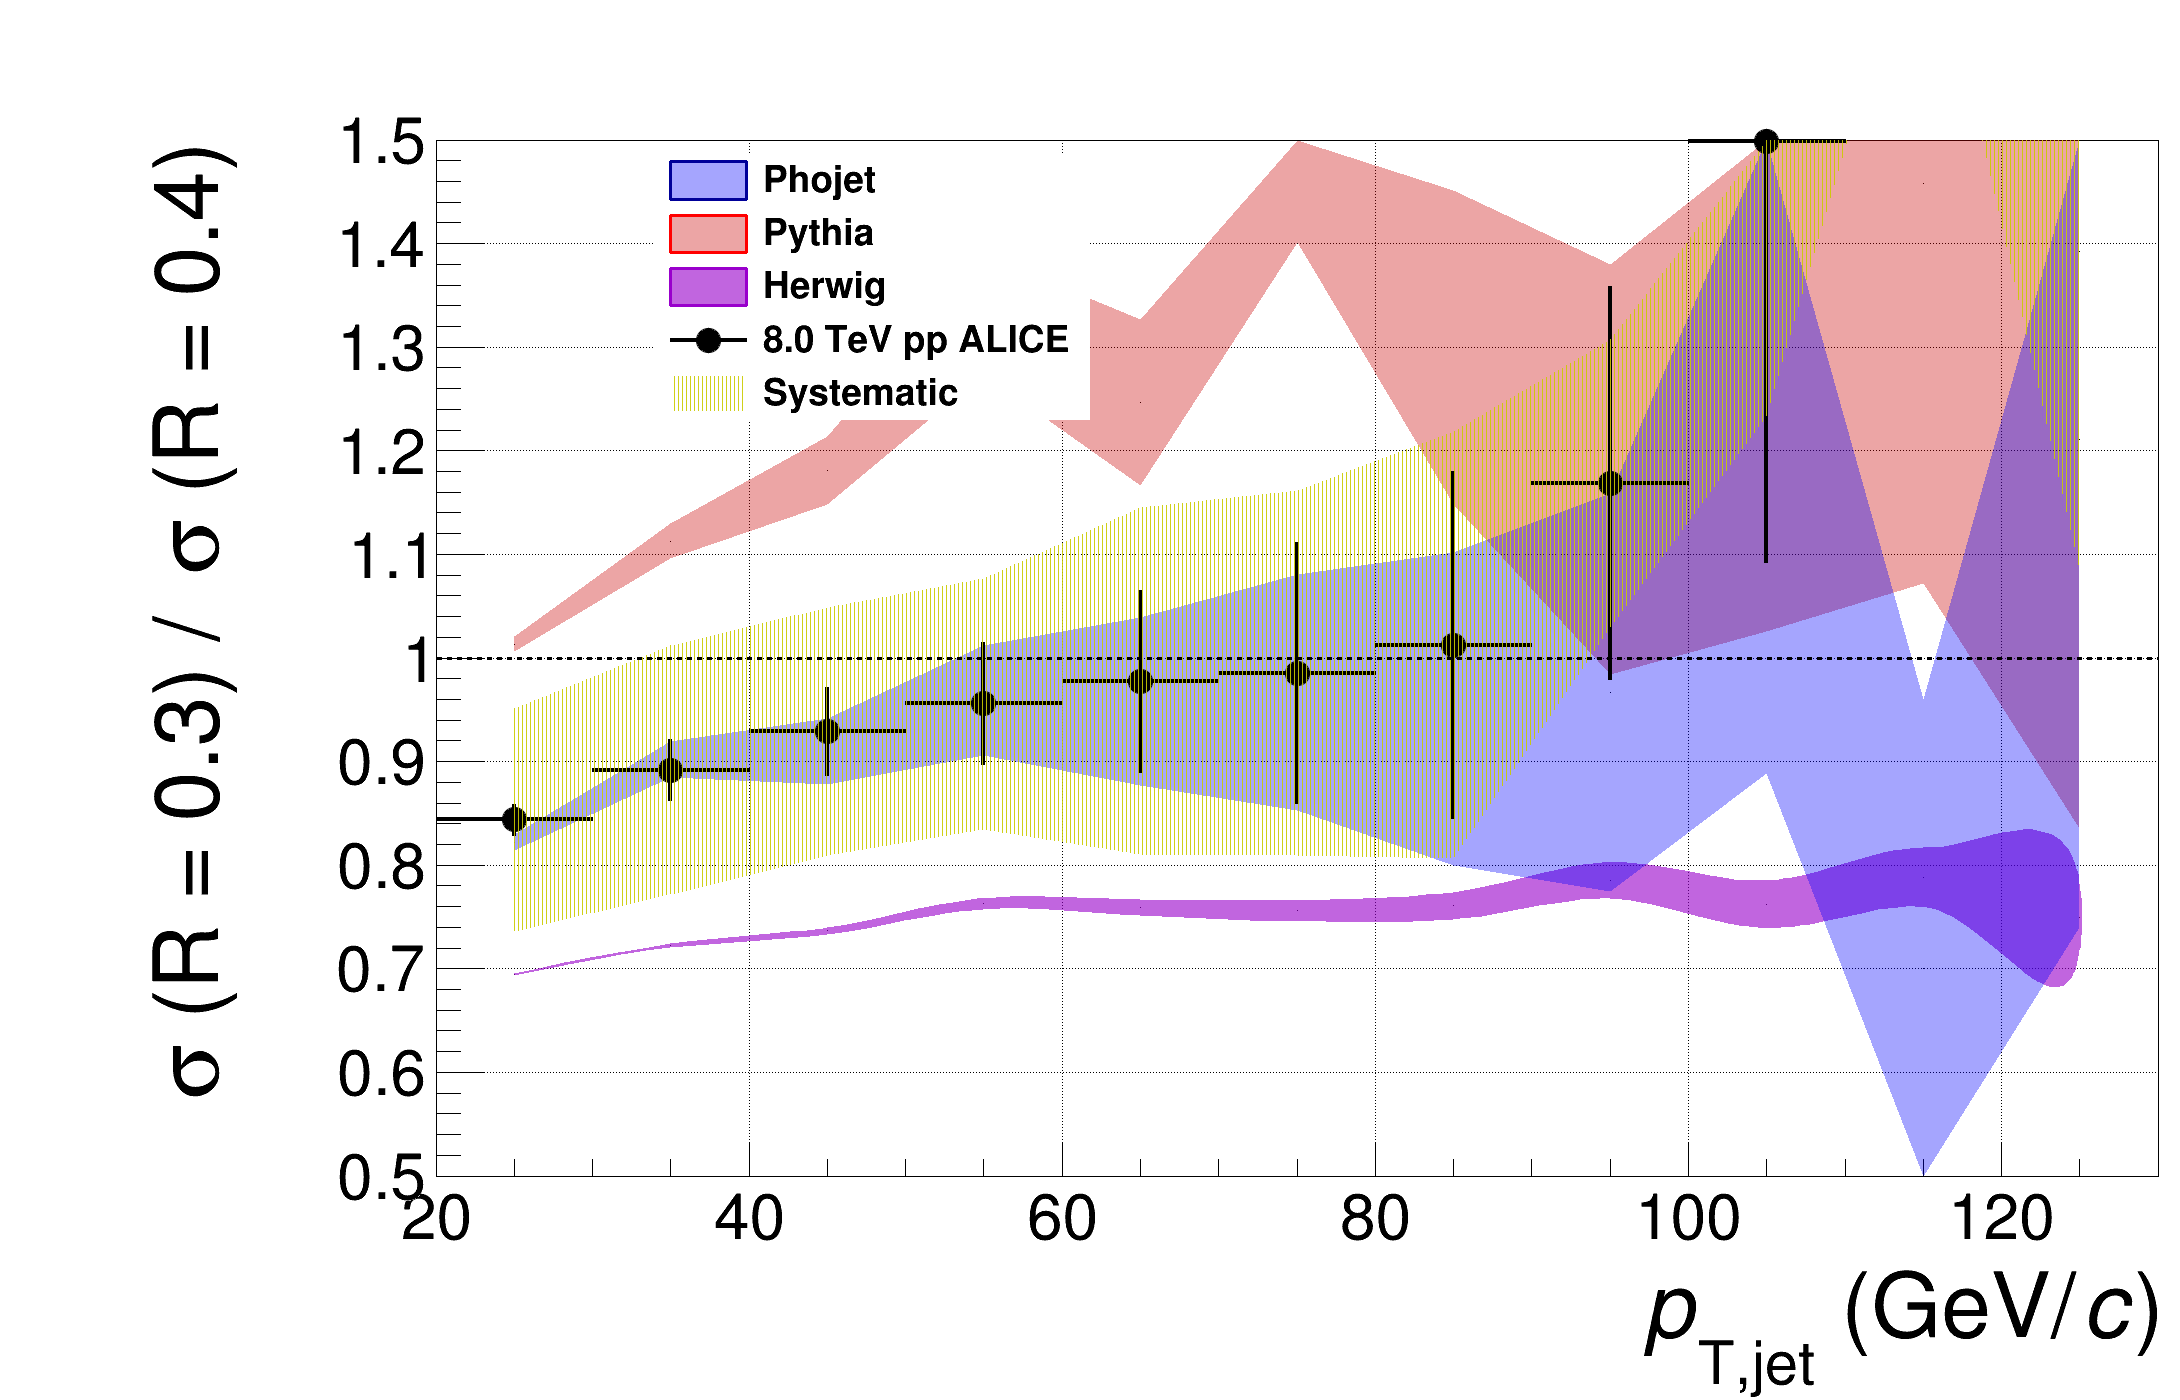
\includegraphics[width=\linewidth]{XSecRatioR03}
\centering
\caption{Ratio of the jet cross-sections R = 0.3  to R = 0.4.}
\label{fig:JetXsecRatioR03}
\end{figure}


\begin{figure}
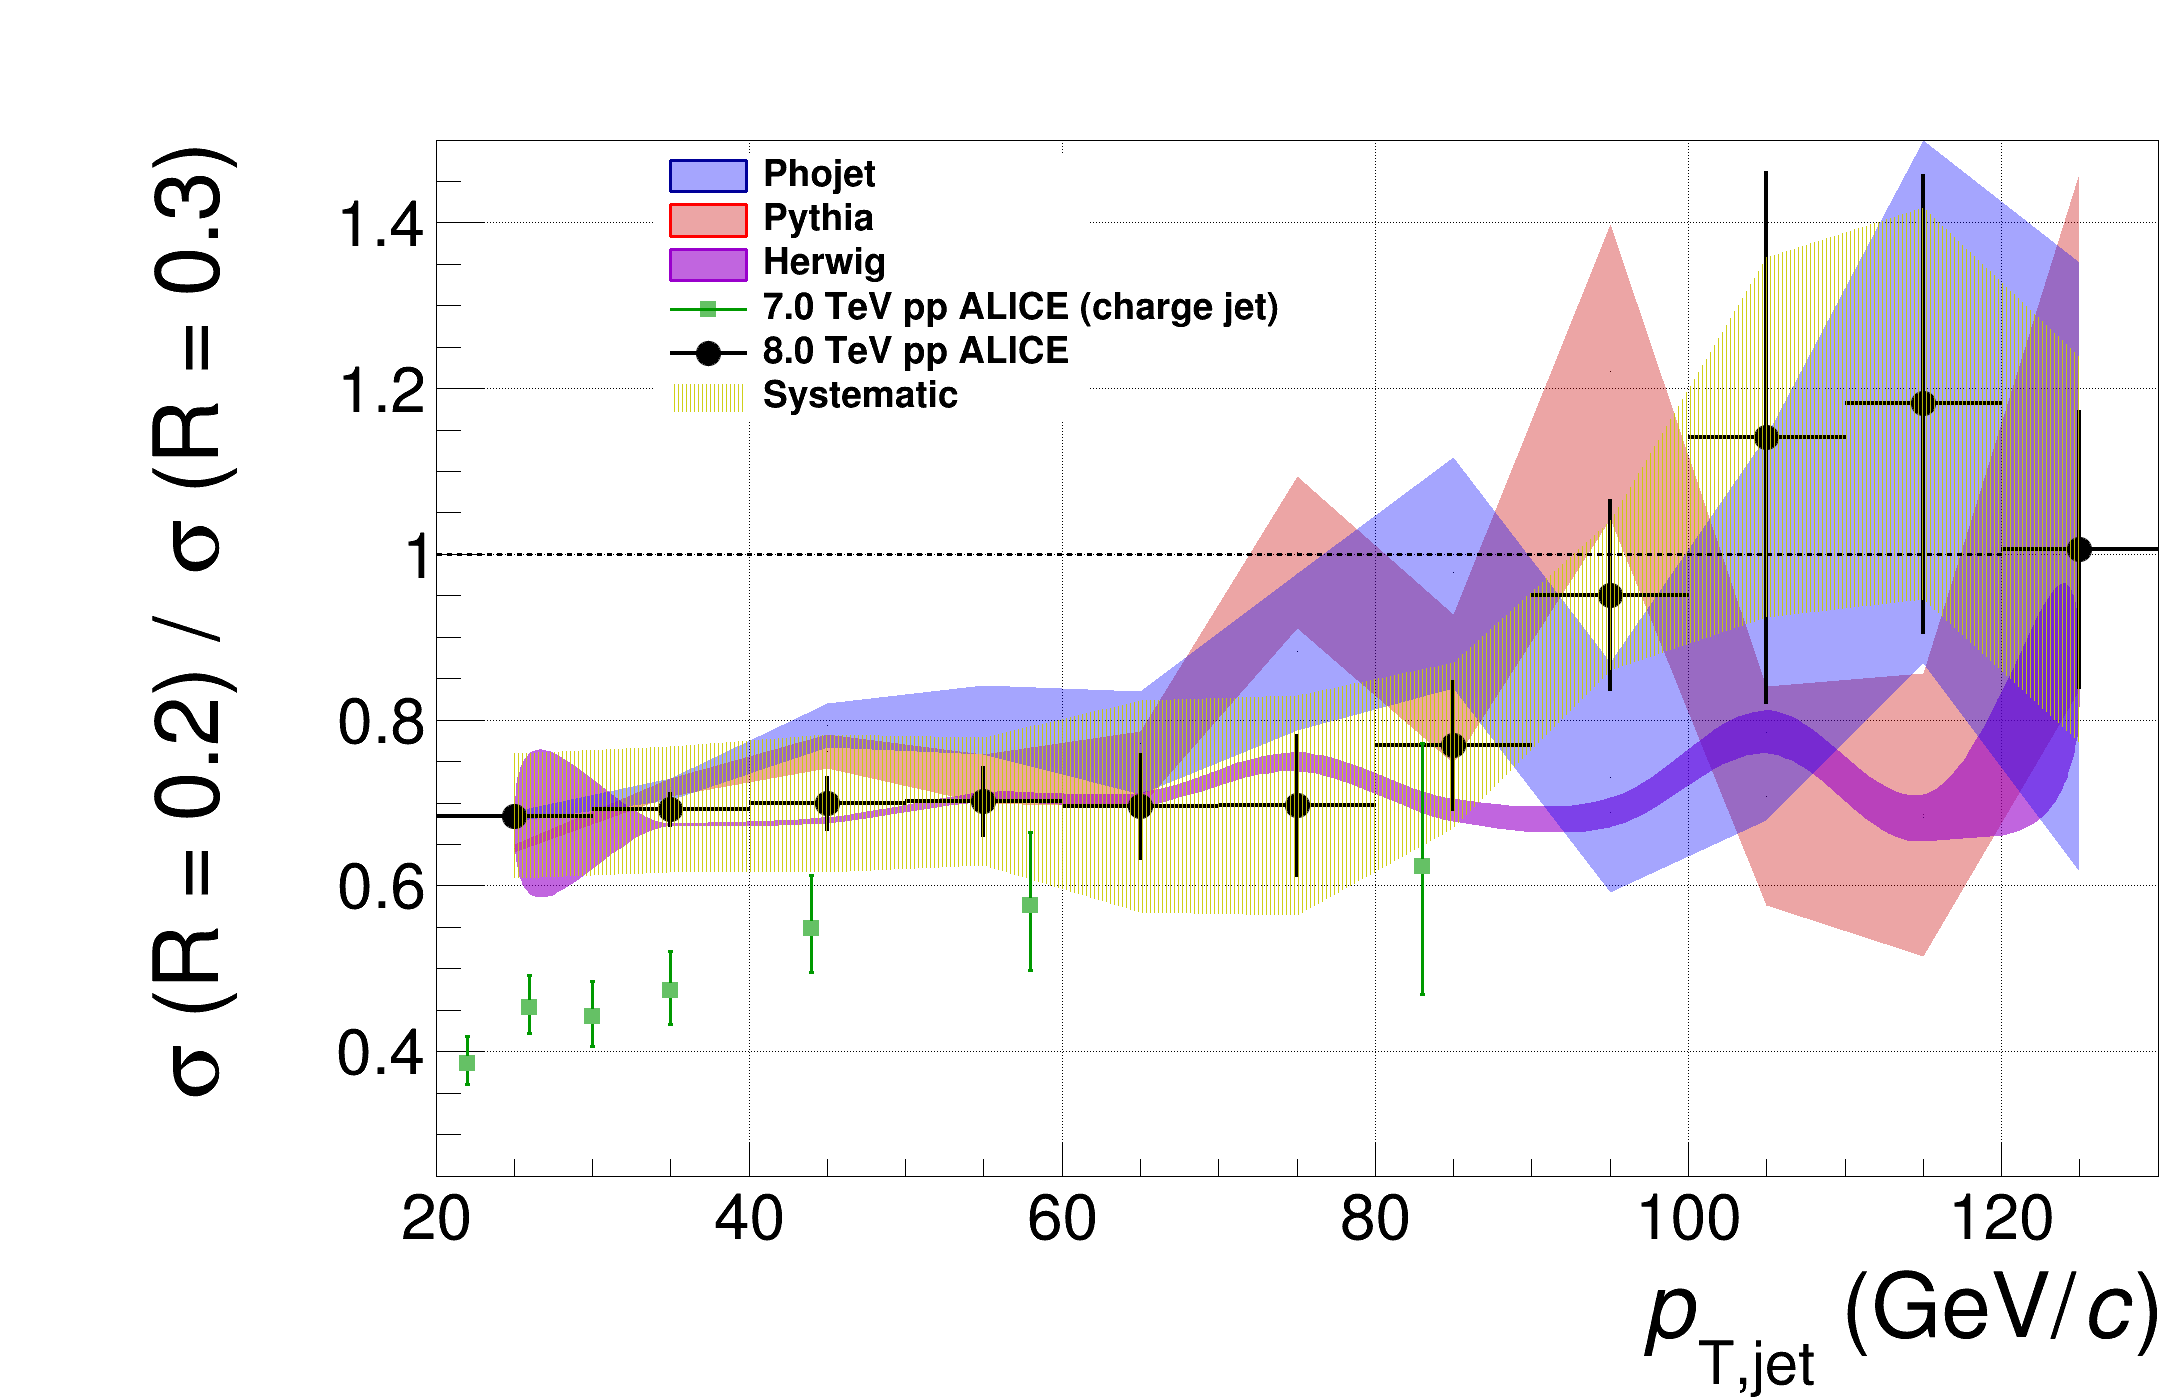
\includegraphics[width=\linewidth]{XSecRatioR023}
\centering
\caption{Ratio of the jet cross-sections R = 0.2  to R = 0.3.}
\label{fig:JetXsecRatioR023}
\end{figure}

\clearpage
}


A similar analysis to this thesis was performed using a 2.76 TeV  data sample collected from ALICE\cite{MA2013319} and it is compared to the 8 TeV data seen in Figure \ref{fig:JetXsecRatioR02}.  ALICE reported a charge jet cross-section ratio between R = 0.2 and R = 0.3 using 7 TeV proton-proton data\cite{Acharya:2018eat} included in Figure \ref{fig:JetXsecRatioR023}.

From the results of the cross-section ratios, we see that the 8 TeV data as reported from this thesis agrees well with the 2.76 TeV results in Figure \ref{fig:JetXsecRatioR02}.  Interestingly it seems that the PHOJET model agrees well with the data for all three figures and is the simulation that agrees the best for the $\sigma (R = 0.3)$ / $\sigma (R = 0.4)$ ratio.  It can be concluded that the PYTHIA ratios have the least agreement because it only includes the LO matrix to calculate partonic showers, which does not model the angular ordering of QCD radiation very well.  HERWIG tends to underestimate the data, especially at low-$p_{T}$, which is expected and may be understood in terms of limitations of modeling low energy background particles with the tune used in this thesis (v2.3).  

These results also report the first ratio of jet cross-sections between R = 0.2 and R = 0.3 at 8 TeV.  This is especially helpful for heavy-ion collisions as most jet results from heavy-ions use either an R = 0.2 or R = 0.3 jet radius to suppress the background in the high multiplicity environment.


\section{Summary and Conclusion}

As two partons undergo a hard scattering they will fragment into collimated sprays of particles known as jets.  Jets are created in the earliest stage of a high energy collision and probe QCD interactions.  Reconstructing full jets in proton-proton collisions also provides an experimental probe of parton kinematics and a baseline for measurements in heavy ion collisions.

This thesis presents the first measurements of inclusive jets at $\sqrt{s} = \,$ 8 TeV using the ALICE detector.  Through the use of the TPC and the EMCal a low level of uncertainty on the jet cross-section was obtained.  In addition, an approach to reconstructing and scaling jets that fired the high-$p_{T}$ EMCal trigger is presented.  By combining the Min Bias and EMCal triggered data we obtained jet measurements over a wide kinematic range.

The agreement between the data and Monte Carlo simulations show that jets are a well calibrated probe for testing QCD.  In terms of the kinematic reach, the results of this thesis agree with simulations between 20 GeV/\textit{c} through 100 GeV/\textit{c} in $p_{T}$.  This range may be extended to 200 GeV/\textit{c} with higher statistics Monte Carlo simulations in the future.  Higher statistic Monte Carlo simulations would also allow for unfolding and correlation studies of the systematic uncertainties.

%The results from this thesis can serve as a baseline measurement for understanding jet quenching in future measurements.   Scaling the obtained cross-sections to heavy-ion energies would allow for new calculations of the nuclear modification factor.  Previous higher energy jet results tended to bias jets to those that traveled a short distance through the Plasma.

In addition to the jet results, this thesis presented the work performed upgrading the ALICE TPC in anticipation of the high luminosity upgrade of the LHC.  The original multiwire proportional chamber design was replaced with a stack of gaseous electron multiplier foils that will allow for a continuous readout of data.  Developing, testing, and production of the new read-out chamber design was performed at the University of Tennessee.

The 8 TeV data are one of the largest data sets and samples jets over a wide kinematic range.  With the LHC, we have moved into high precision measurements of QCD phenomena using rare probes such as jets.  The work in this thesis sets the stage for using jets with ALICE in the future.  
% What results we will gain from the upgraded LHC and jets is only left to our imagination and to nature's mercy.


